% В этом шаблоне используется класс spbau-diploma. Его можно найти и, если требуется, 
% поправить в файле spbau-diploma.cls
\documentclass{spbau-diploma}
\begin{document}
% Год, город, название университета и факультета предопределены,
% но можно и поменять.
% Если англоязычная титульная страница не нужна, то ее можно просто удалить.
\filltitle{ru}{
    chair              = {Кафедра математических и информационных технологий},
    title              = {Вычислительное моделирование посттравматического нейрогенеза},
    % Здесь указывается тип работы. Возможные значения:
    %   coursework - Курсовая работа
    %   diploma - Диплом специалиста
    %   master - Диплом магистра
    %   bachelor - Диплом бакалавра
    type               = {master},
    position           = {студента},
    group              = 602,
    author             = {Мыров Владислав Олегович},
    supervisorPosition = {???},
    supervisor         = {Божко Дмитрий},
    reviewerPosition   = {???},
    reviewer           = {???},
    chairHeadPosition  = {д.\,ф.-м.\,н., профессор},
    chairHead          = {Омельченко А.\,В.},
    % university = {САНКТ-ПЕТЕРБУРГСКИЙ АКАДЕМИЧЕСКИЙ УНИВЕРСИТЕТ},
    % faculty = {Центр высшего образования},
    % city = {Санкт-Петербург},м
    % year             = {2013}
}
\filltitle{en}{
    chair              = {Department of Mathematics and Information Technology},
    title              = {Computational modelling of post-traumatic neurogenesis},
    author             = {Myrov Vladislav},
    supervisorPosition = {???},
    supervisor         = {Dmitriy Bozhko},
    reviewerPosition   = {???},
    reviewer           = {???},
    chairHeadPosition  = {professor},
    chairHead          = {Alexander Omelchenko},
}
\maketitle
\tableofcontents
% У введения нет номера главы
\section*{Введение}
Травмы головного мозга являются серьезной угрозой здоровью, которая может вызвать недееспособность или нетрудоспособность. Не смотря на развитие хирургических методов лечения, но эффективной восстановительной терапии, особенно при потери когнитивных навыков, пока нет.

В современной фармацевтике вычислительные модели стали необходимым первичным этапом разработки лекарства, поскольку позволяют предсказать возможное течение лечения и его результаты. Так же они ускоряют и сильно удешевлеяют предварительные испытания потому что снижается необходимость в экспериментах in vivo, которые трудоемки и дороги, особенно в случаях исследований нервной ткани. 

Современные модели нейронной популяции сконцентрированы на передаче нейронных импульсов между клетками, уделяя меньше внимания биохимическим процессам, происходящим в них. В свою очередь, именно эти процессы наиболее интересны при разработке лекарств. Так же интересен не только результат лечения, но и то как можно повлиять на него, изменяя различные параметры. Эти факторы приводят к необходимости разработки вычислительной модели, которая позволит не только учесть биохимические реакции, происходящие в нервной ткани, но и подобрать такие параметры воздействия на модель, что результат будет наиболее эффективным.

В данной работе я представляю модель нейрогенеза, основанную на эволюционной модели нервной активности.

\section{Описание модели}

To fill...

\section{Дизайн экспериментов}

Для экспериментов было выделено три основных типа повреждений:

\begin{enumerate}
    \item Травмы. Данный тип повреждений получен после некоего повреждения извне, например падения, удара головой о твердую поверхность. Характеризуется локальностью повреждений, но относительно большим объемом \cite{genesis_trauma}. Для симуляции травмы случайно выбирается точка на поверхности нервной ткани и уничтожается заданный процент нейронов в окрестности точки.
    \item Инсульт. Характеризуется многочисленными, но небольшими повреждениями, которые могут быть расположены по большому объему ткани\cite{genesis_stroke}. Для симуляции инсульта случайно выбираются нейроны в ткани и уничтожается небольшое число случайных клеток в их окрестности пока не будет будет уничтожен заданный процент популяции.
    \item Возрастные изменения. Характеризуются смертью не только нейронов, но и деградацией соответствующих механизмов, которые могут выражаться в уменьшении числа стволовых клеток, замедленного роста синапсов\cite{genesis_aging}. Симуляция возрастных измненений производится в непрерывной, но медленной смерти всех клеток.  
\end{enumerate}

Так же для экспериментов для каждого типа повреждений были проведены эксперименты где умирали клетки только определенного типа.

В экспериментах исследовалась завимость между качеством обучения популяции нейронов и количеством нейронов в популяции. Так же проводилось исследование не только зависимости от количества нейронов, но и структуры которую популяция образовывала. Так же проводились исследования того как нейрогенез зависит от расположения стволовых клеток: расположены ли они равномерно по всей ткани, сконцентрированы ли в единой точке или имеют другое, например нормальное вокруг некоей точки, распределение.

Эксперименты с травмами проводились следующими шагами:

\begin{enumerate}
    \item Изначальное обучение модели.
    \item Первая проверка ее качества на независимой выборке, получение базового уровня.
    \item Нанесение повреждений согласно типу эксперимента.
    \item Проверка качества модели поврежденной ткани, наблюдается ли деградация.
    \item (опционально) добавление некоего фармакологического агента, который может стимулировать или тормозить нейрогенез.
    \item Процесс нейрогенеза пока ткань не сойдется к стабильному с точки зрения топологии состоянию.
    \item Третья проверка качества модели и сравнение топологий до повреждений и после.
\end{enumerate}

Обобщенная схема экспериментов с травмами представлена на рисунке 1.

\begin{figure}[h]
\centering
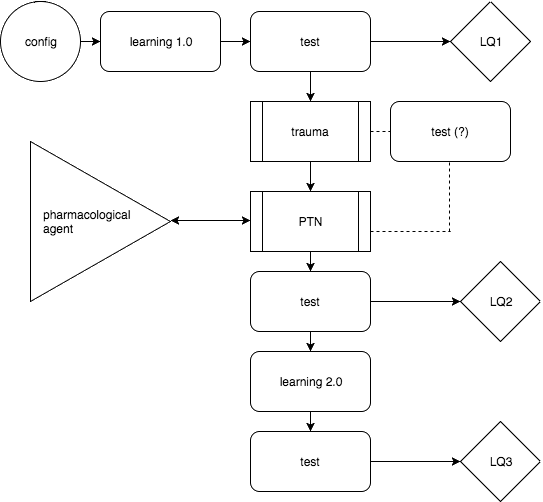
\includegraphics[scale=0.5]{images/testing_scheme.png}
\caption{Схема эксперимента}
\label{testing_scheme}
\end{figure}


В случае возрастных изменений эксперимент похож на обучение модели, но с постепенной смертью всех клеток. В данном случае поскольку клетки умирают не однократно, а в течении всей жизни модели, нельзя выделить единый этап нанесения повреждений и восстановления. Поэтому замеры качества обучения проводятся на протяжении всего эксперимента и основной интерес представляет собой динамика. Сводная таблица с описаниями экспериментов представлено в таблице \ref{tab:experiments}, описание параметров представлено в таблице \ref{tab:exp_params}.


\begin{table}
    \centering
    \begin{tabular}{ | p{2.5cm} | p{3.5cm} | p{5cm} | p{2cm} |}
    \hline
    Тип эксперимента & Параметры & Выбор нейронов & Процент травмированных тканей \\ \hline
    Травмы & Типы нейронов: сенсорные, внутренние, нейроны принятия решений, объем травмы. & Единовременно выбирается точка, потом в ее окрестности набирается необходимое число клеток. В зависимости от типа повреждаемой ткани, варьируется место травмы. & 5-20\% \\ \hline
    Инсульт & Типы нейронов: сенсорные, внутренние, нейроны принятия решений, объем повреждений. & Выбирается нейрон и повреждается несколько в его окрестности. Данная процедура повторяется пока не наберется необходимая масса & 5-15\% \\ \hline
    Возрастные изменения & Вероятности умереть заданному типу клетки. В данном эксперименте умирают не только нейроны, но и стволовые клетки, глиальные. скорость с которой происходит смерть. & С заданной периодичностью выбирается случайная клетка и погибает & 0-100\% \\
    \hline
    \end{tabular}
    \label{tab:experiments}
\end{table}


\begin{table}
\centering
    \begin{tabular}{ | p{2.5cm} | p{3.5cm} | p{3cm} | p{4cm} |}
    \hline
    Параметр & Возможные значения & Тип параметра & Эксперименты \\ \hline
    Тип нейронов & Сенсорные, внутренние, нейроны принятия решений. & Дискретный & Травма, инсульт, возрастные изменения \\ \hline
    Объем повреждений & 0-100\%. & Непрерывный & Травма, инсульт. \\ \hline
    Тип клеток & Все типы нейронов (3), глиальные и стволовые клетки & Дискретный & Возрастные изменения \\ \hline
    Распределение стволовых клеток & Равномерное по ткани, равномерно по окрестности, нормальное & Дискретный & Травма, инсульт, возрастные изменения \\ \hline
    Тип выбора клеток & Случайно равномерно, равномерно по окрестности, нормально & Дискретный & Возрастные изменения, инсульт \\ \hline
    Выбор места травмы & Случайно равномерно, равномерно по окрестности, нормально (в случае травмы выбираются точки только на поверхности) & Дискретный & Инсульт, травма \\ \hline
    \end{tabular}
    \label{tab:exp_params}
\end{table}



% \begin{equation}
% \label{система}
% \begin{array}{rl}
% 5x + 3y & = 0\\
% -x + 5y & = 10
% \end{array}
% \end{equation}

% Рисунок, размещенный с предпочтением "вверху страницы"
% \begin{figure}[t]
% \centering
% \includegraphics{fig1.jpg}
% \caption{Разрыв функции}
% \label{разрыв_функции}
% \end{figure}


% У заключения нет номера главы
\section*{Заключение}


\bibliographystyle{ugost2008ls}
\bibliography{diploma.bib}
\end{document}
